
%----------------------------------------------------------------------------------------
%	PACKAGES AND OTHER DOCUMENT CONFIGURATIONS
%----------------------------------------------------------------------------------------

\documentclass[paper=a4, fontsize=9px]{scrartcl} % A4 paper and 11pt font size

\usepackage[T1]{fontenc} % Use 8-bit encoding that has 256 glyphs
\usepackage{fourier} % Use the Adobe Utopia font for the document - comment this line to return to the LaTeX default
\usepackage[UTF8]{inputenc}
\usepackage[english]{babel} % English language/hyphenation
\usepackage{amsmath,amsfonts,amsthm} % Math packages

% Scaling < and >
\usepackage{scalerel}
\usepackage{multicol}

\usepackage{listings}
\usepackage{courier}
\usepackage{minted}
\usepackage[section]{placeins}
\usepackage{hyphenat}

\hyphenation{key-words}


%\usepackage{algorithm2e}
%\lstset{basicstyle=\scriptsize\ttfamily,breaklines=true}
\lstset{framextopmargin=0pt,frame=topbottom,numbers=left,mathescape=true}

\usepackage{lipsum} % Used for inserting dummy 'Lorem ipsum' text into the template

\usepackage{graphicx}
\usepackage{enumitem}
\usepackage{hyperref}

\usepackage{calrsfs}
\DeclareMathAlphabet{\pazocal}{OMS}{zplm}{m}{n}

% Tikz
\usepackage{tikz, amssymb, bm, color}
\usetikzlibrary{shapes,arrows}

\usepackage{sectsty} % Allows customizing section commands
\allsectionsfont{\centering \normalfont\scshape} % Make all sections centered, the default font and small caps

\usepackage{fancyhdr} % Custom headers and footers
\pagestyle{fancyplain} % Makes all pages in the document conform to the custom headers and footers
\fancyhead{} % No page header - if you want one, create it in the same way as the footers below
\fancyfoot[L]{\thepage} % Empty left footer
\fancyfoot[C]{} % Empty center footer
\fancyfoot[R]{} % Page numbering for right footer
\renewcommand{\headrulewidth}{0pt} % Remove header underlines
\renewcommand{\footrulewidth}{0pt} % Remove footer underlines
\setlength{\headheight}{13.6pt} % Customize the height of the header

\usepackage[margin=1.0in]{geometry}

\numberwithin{equation}{section} % Number equations within sections (i.e. 1.1, 1.2, 2.1, 2.2 instead of 1, 2, 3, 4)
\numberwithin{figure}{section} % Number figures within sections (i.e. 1.1, 1.2, 2.1, 2.2 instead of 1, 2, 3, 4)
\numberwithin{table}{section} % Number tables within sections (i.e. 1.1, 1.2, 2.1, 2.2 instead of 1, 2, 3, 4)

%\renewcommand{\theenumii}{\arabic{enumii}}

%\setlength\parindent{0pt} % Removes all indentation from paragraphs - comment this line for an assignment with lots of text

%----------------------------------------------------------------------------------------
%	TITLE SECTION
%----------------------------------------------------------------------------------------

\newcommand{\horrule}[1]{\rule{\linewidth}{#1}} % Create horizontal rule command with 1 argument of height

\title{	
\normalfont \normalsize 
\textsc{University of Twente --- Managing Big Data} \\ [5pt] % Your university, school and/or department name(s)
\horrule{0.5pt} \\[0.4cm] % Thin top horizontal rule
\huge Relation between Dutch news coverage and climate awareness on Twitter \\ % The assignment title
\horrule{2pt} \\[0.0cm] % Thick bottom horizontal rule
}

\author{{\small \textsc{Ivaylo Hristov} (\texttt{i.hristov@student.utwente.nl})}\\{\small \textsc{Hidde Wieringa} (\texttt{hidde@hiddewieringa.nl})}\\{\small \textsc{Sebastian Panman de Wit} (\texttt{j.s.panmandewit@student.utwente.nl})}} % Your name
\date{\normalsize\today} % Today's date or a custom date

% Fix figure environment in multicol
\newenvironment{Figure}
{\par\medskip\noindent\minipage{\linewidth}}
{\endminipage\par\medskip}

\newcommand{\diff}{\,\text{d}}
\newcommand{\G}{\pazocal{G}}
\newcommand{\N}{\mathbb{N}}
\newcommand{\god}{\text{göd}}
\newcommand{\godinv}{\ensuremath{\text{göd}^{-1}}}
\newcommand{\REC}{\mathsf{REC}}
\newcommand{\R}{\mathbb{R}}
\newcommand{\I}{\mathbf{I}}
\newcommand{\LS}{LS}
\newcommand{\cont}{\pazocal{C}}
\newcommand{\C}{\mathbb{C}}
\newcommand{\proj}[2]{\pazocal{P}_#1(#2)}

\newcommand{\norm}[2]{\left\lVert#1\right\rVert_{#2}}
\newcommand{\seq}[1]{\underbar{{#1}}}
\newcommand{\conj}[1]{\overline{#1}}
\newcommand{\ddx}[1]{\frac{\diff #1}{\diff x}}

\begin{document}

\maketitle % Print the title
%\pagestyle{empty}

\begin{multicols}{2}

\section{Introduction}

Since 1880 to 2012 the average global temperature increased by by 0.85\% [1]. This has lead to the United Nations setting one of their goals to take immediate action to climate change. One way to do this is by first increasing climate awareness [2]. According to one study [3], public awareness of global warming issues increased after an increase in media coverage of global warming. These results were based on a survey of 2000 respondents. Big data techniques used in combination with data from social media however can provide us with a bigger sample to measure the public awareness of global warming issues. Multiple other studies have been conducted to measure the influence of news coverage on social network activity like Twitter[4][5], however little research has been done in finding a relation between news coverage and climate awareness on social network.

This paper therefore explores the relation of climate awareness on social media and news articles about the climate by using big data techniques on data from social media. To narrow down the total data and due to time constraints, only Twitter data will be used measure the climate awareness on social media. Using big data techniques and Twitter data is a valuable way to observe people opinion on climate changes [6], so this reduction of our scope will not affect the value of our result. For the news articles, articles from the Volkskrant will be used to measure the media coverage because of time constraints. The data is stored on a Hadoop Filesystem (HDFS). We use Spark to filter the data to find relevant articles and tweets. Over a time period of 5 years (2011 until and including 2015) the data is grouped into smaller time intervals. Afterwards a statistical analysis will be performed to find a correlation between the news articles and tweets concerning climate change. If a correlation is found then this is a sign of a relation between news articles and tweets concerning climate change, although multiple causes can be thought of which explain the correlation. A positive correlation shows that an increase in the amount of news coverage of climate related subjects increases climate awareness on social media or vice versa.

Section \ref{sec:method} explains the data used and the methods to filter out the relevant data. This section also provides the way we performed the statistical analysis.
Afterwards in section \ref{sec:results} the results of the process of classifying the data are provided. In section \ref{sec:conclusion} we will summarize our finding and provide a conclusion to our research. Finally, in section \ref{sec:limitations} we discuss the limitations of this research and provide further research subjects.


\section{Materials and Method}\label{sec:method}

A brief description of all materials and methods used in this research will be given. The datasets, the process of classifying the data as climate related, the used technology, the verification of the results and finally the used statistics to formulate the results will all be explained.


\subsection{Datasets}

Three datasets have been used for this research, namely news articles of the Volkskrant, tweets from Twitter and a list of climate related keywords.

For the news items, articles from the Dutch website of Volkskrant have been taken. The news articles in our dataset have been published between 2010 up to and including 2016 (a total of 491,852 articles; size on disk 9.7GB compressed, 29.1GB uncompressed). The articles are split into multiple JSON files with information of the title, publishing timestamp, category, and content. The length of the content (title and text) of the news articles ranges from 0 characters to 87,328 characters. Because the range of the length of the content of the articles is so large, the statistics we deduce later are all per 1000 words of content. 


The second dataset is Dutch Twitter data, which has been selected, and preprocessed by Tjong Kim Sang et al [7]. The data ranges from 1 January 2011 up to and including 31 December 2011, a total number of 4,308,911,953 tweets, taking 1.6 TB on disk compressed and 4.9 TB uncompressed. The dataset includes a large number of metadata fields which are not used: only the text content and the timestamp of publishing of the tweet are used. Data extraction of the tweets was however not trivial because the structure of the dataset is not the same throughout the dataset. This meant that while the data could not be viewed manually (it is terabytes large), the structure had to be determined programmatically. Also sometimes timestamp field `timestamp\_ms’ could not be used (it was absent) so the field `created\_at’ must be used. That field contained a textual representation of the timestamp which must be parsed again to useful information. However, there was also a time zone present (always `+0000’) of which there is no support in Python 2.7 without extensions. After removing the time zone information, the timestamp could be parsed and the time information was almost complete. There still remained some tweets witch had neither a `timestamp\_ms’ nor a `created\_at’ field. These tweets usually also had no content so they have been discarded due to invalidity. 

The overlapping time period of the two datasets is 16-01-2011 until and including 30-11-2015. This includes 391,249 news articles and 4,241,945,655 tweets.

Lastly we used a list of keywords related to climate which we found on the internet\footnote{Source: \url{https://sustainability.unc.edu/files/2015/12/Sustainability-Keywords.pdf}}. This list was not optimal for our use because it was written in English so some edits had to be made to be able to use it for classification of the Dutch text in our datasets. First of all the list has been translated into Dutch electronically and afterwards corrected manually where needed. Some other adjustments had to be made which included removing stopwords, removing ambiguous words, and adding the plural/singular form of keywords. Fortunately a lot of terms which consisted of multiple words in English usually became a single word in Dutch, which simplified matching the terms during the classification process. 

For the full list of terms, both the English and Dutch version, see the appendix.

\begin{Figure}
	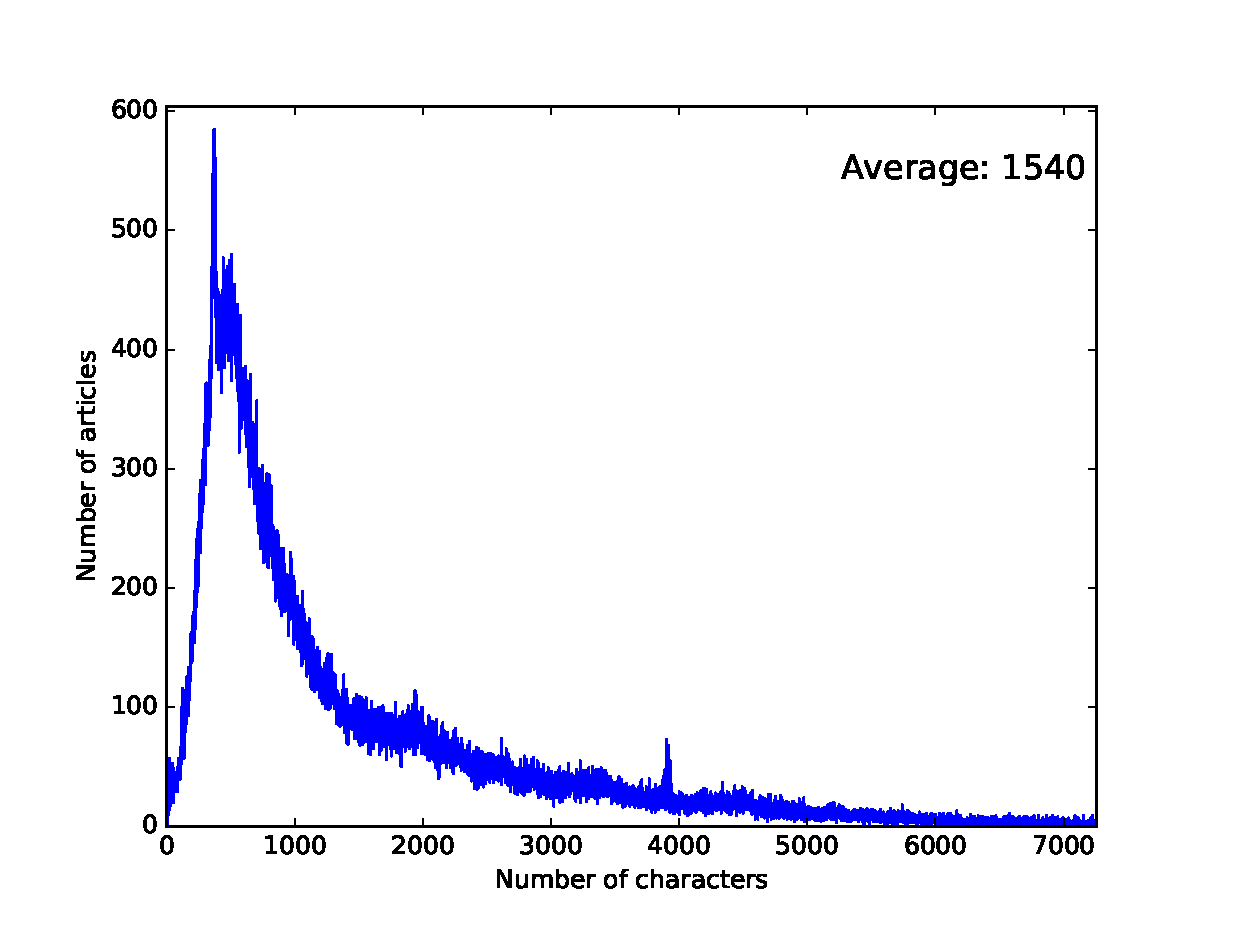
\includegraphics[width=\textwidth]{img/articles_characters}
	\captionof{figure}{The number of Volkskrant articles with a certain number of characters.}\label{fig:9}
\end{Figure}



\subsection{Classification of text}

The content of news articles and tweets needs to be classified as either related to climate or not, to count the number of climate related articles and tweets. Different techniques are possible [4] but due to the time constraint a relative easy classification has been used. We used the list of keywords related to climate, to count the matches of keywords (related to climate) in the articles and tweets

The thresholds are different for the articles and the tweets since these differ in amount of characters of content. 

For each tweet and article, we count the number of occurrences of a keyword (related to climate) in the title and text. If the count is above the threshold, then the news article or tweet is `climate related’. To determine this threshold, we analysed the frequency distribution of the amount of keywords in the news articles and tweets, and selected the threshold for each data source such that around less than 5\% qualifies as `climate related’, and there are enough articles/tweets in the remaining dataset. We chose the threshold for the Volkskrant articles at 5 per 1000 words which resulted in 3.6\% of the articles being rated as `climate related'. For Twitter we required 3 or more keyword matches to classify the tweet as `climate related, which resulted in 0.02\% of all tweets.

Initially, we defined a title factor for the news articles. We expected that terms occurring in the title of a news article have more impact for raising climate awareness. The matches of any terms in the title of a news article are thus multiplied with a factor. Unfortunately, due to time constraint, we did not use this.

\begin{Figure}
	\includegraphics[width=\textwidth]{img/threshold_twitter_log_scale}
	\captionof{figure}{The number of tweets with a certain amount of keyword matches.}\label{fig:1}
\end{Figure}

\begin{Figure}
	\includegraphics[width=\textwidth]{img/threshold_volkskrant_log_scale}
	\captionof{figure}{The number of Volkskrant articles with a certain amount of keyword matches.}\label{fig:2}
\end{Figure}

\subsection{Technology}\label{sec:technology}

To store the data, a server cluster has been used with a Hadoop File System (HDFS) to manage the storing, replication, and retrieval of data. On top of the HDFS we can process the data using Spark (specifically PySpark). The extended functionality SparkSQL has been used which allows easier reading of data in JSON format, and the use of SQL statements to manipulate data. 
To process a Python 2.7 script on the server cluster, Yarn is used to manage the cluster, to copy and execute the Python code on the nodes, and to retrieve the results. 

To represent the data visually we have plotted the extracted data from the cluster using the matplotlib package for Python. A problem arising was that the data was not JSON formatted but there were only tuples (a type of Python object).  This meant that we had to parse the output files.

After the data from the output file had been parsed we formatted and filtered it the way we required. Using this, we have created plots of the data to visualize it, using the library matplotlib. Also various statistics have been added such as the average, the standard deviation, the correlation coefficient (when two datasets are plotted). We did not have to implement the different formulas to calculate the statistics by hand, but could calculate them with help of the numerical scientific python package NumPy. With these statistics we were able to examine the data with different thresholds and search for peaks of news/tweets that are relevant to our research.

To verify the data and the visualisation of it with Python, we used Excel. The dataset in Excel was put into a large Pivot Table. Using this feature of Excel allowed us to plot the same figures as in Python and then to check whether these were similar. Also the numbers could be verified using this feature. 
Another benefit of using Pivot Tables in Excel was that it allowed us to quickly manipulate the data by filtering, summing, grouping and filtering the data any required way. This made looking at the impact of different adjustments to the dataset easier than it would have been in NumPy. These different adjustments were for example adjusting thresholds and time periods. From this we decided the different thresholds based on our requirements on the number of articles and tweets, and then used Python to plot figures in more detail. Also the statistical analysis in Python has been verified using the statistical analysis tool in Excel.



\subsection{Verification}

To verify our results, news articles related to climate change have been used from the NOS which we found manually. The verification of the classification of the tweets/articles has been done by visualizing the classification over time, and then analysing the visualisation(s) in detail. Also, the top matching articles and tweets were extracted from the cluster to view the content and verify the climate-relatedness. Both datasets have been verified to make sure that any conclusions drawn from these datasets are relevant and correct.

The chosen visualisation was a line plot of the data over time (like figures \ref{fig:3} and \ref{fig:4}), with the value the sum of the number of articles or tweets on that date. Optionally, a threshold could be added such that only articles or tweets which match more terms than the threshold are included in the sum.

After plotting the data over time, a number of peaks are present (figures \ref{fig:5} and \ref{fig:6}). Sometimes the peaks are not absolute peaks (the largest values over all time), but relative peaks (an outlier in that period of time). Using these peaks, the classification is verified manually in two ways: the existing peaks are verified with actual climate-related events, and climate-related events are checked to cause peaks in the visualisation.

To verify a peak in the plot, the time range of a few dates before or after the date of the peak have been looked up on the website of NOS. For a peak to exist and be verified, there must be some corresponding climate related events around the same date as the peak.

Also pre-selected climate related events (the yearly UN Climate change Conferences) were looked into to find the date of the event, and verify that a peak exists in the plot of the data. 

This verification was executed twice for each dataset. First the peaks were analysed with the threshold at a high level, such that only a few top tweets/articles were shown. After all, top tweets or articles should match a climate related event. Then, the normal thresholds were used to verify those tweets and articles that caused peaks. After all, tweets and articles with a high count should also match a climate related event.



\subsection{Statistics}

The total counts of the number of tweets and news articles qualified as `climate related’ (which means the number of matches to terms is above the chosen threshold) have been grouped per day over the time period where data exists for both datasets. These two time series have been correlated to find a correlation factor: first for all the data to get a baseline correlation, and then for only the climate-related articles and tweets to see improvement. The numeric calculations are done by the Python package NumPy.

We have also grouped the data by week instead of by day, but the standard deviation became so large that no peaks were visible in the resulting visualisation. This approach has been discarded as ineffective.

\section{Results}\label{sec:results}

The results are described per step in the processing of the data. All code to process the data and the useful output which represents our results can be found in the GitHub repository\footnote{\url{https://github.com/electrofLy/big\_data\_climate\_change}}.


\subsection{Classification}

The classification of the raw Twitter and Volkskrant data gave us the input data for the rest of the research. This means that the raw dataset has been filtered for the overlapping time frame, and output grouped by date and number of matches. Per date and number of matches we then have  a count. 

With these counts we were able to determine a threshold for rating articles and tweets as climate related. In figure \ref{fig:5}, \ref{fig:6} and \ref{fig:8} are a number of visualisations of this data, visualised using the matplotlib package as described in the section \ref{sec:technology}.


\subsection{Verification}

We have done the verification of the resulting data after applying our classification. We noticed a number of things which were not correct with the results. This made us conclude the verification of our results failed and so the results are invalid. Below the verification is outlined in more detail.

To start, the top articles and tweets were extracted from the cluster by filtering by the the largest numbers of matches, such that only a few articles or tweets remained. These have been read manually to check the content for climate relatedness. This resulted in 87 articles (more than 50 matches in the article, in total; not per 1000 words) and 14 tweets (more than 7 matches of keywords). Although a few articles and tweets of those selected top ones were climate related, most were weather related. This might be logical, as many climate issues are also related to weather in terms of keywords.

Some correct matches: 
\begin{itemize}
	\item \textsc{Volkskrant} `Opklaringen in de broeikas’ (`Clear skies in the greenhouse’) 21 September 2013.\footnote{\url{http://www.volkskrant.nl/archief/opklaringen-in-de-broeikas~a3513501/}}
	\item \textsc{Volkskrant} `De dreigende kernramp in Japan vandaag van minuut tot minuut` (`The approaching threatening nuclear disaster in Japan today from minute to minute’) 16 March 2011.\footnote{\url{http://www.volkskrant.nl/buitenland/de-dreigende-kernramp-in-japan-vandaag-van-minuut-tot-minuut~a1860793/}}
	\item \textsc{Twitter} `@Maarijex  ena natuurlijk mooi weer zon zon zon zon zon zon ;k;k;k`
\end{itemize}

Some incorrect matches:
\begin{itemize}
	\item \textsc{Volkskrant} `De volledige tekst van de Troonrede’ (`the complete Troonrede text’) 18 September 2012.\footnote{\url{http://www.volkskrant.nl/politiek/de-volledige-tekst-van-de-troonrede~a3318354}}
	\item \textsc{Volkskrant} `Dankuwel, crisis’ (`Thank you Crisis’) 11 June 2013.\footnote{\url{http://www.volkskrant.nl/archief/dankuwel-crisis~a3456355/}}
	\item \textsc{Twitter} `Denken denken denken en denken denken denken denken denken en oja ook nog denken denken. Maar toch ook wel klein beetje denken hoor.’

\end{itemize}
Next, the peaks of the data filtered with the thresholds have been verified. The relative peaks (around 10 peaks per dataset) have been collected by date and number of articles/tweets. See figures \ref{fig:11} and \ref{fig:10}.


\begin{Figure}
	\centerline{\begin{tabular}{rr}
	Date       & Number of articles \\ \hline
	13/06/2012 & 12                 \\
	17/06/2011 & 11                 \\
	01/10/2011 & 11                 \\
	22/05/2012 & 11                 \\
	18/09/2012 & 11                 \\
	23/10/2012 & 11                 \\
	13/12/2012 & 11                 \\
	01/02/2013 & 11                 \\
	18/05/2013 & 11                 \\
	11/06/2013 & 11
\end{tabular}}
\captionof{figure}{The peaks of the number of articles per day which have a number of keyword matches above the threshold.}\label{fig:11}
\end{Figure}

\begin{Figure}
	\centerline{\begin{tabular}{rr}
			Date       & Number of tweets \\ \hline
			24/05/2012 & 1022               \\
			20/01/2013 & 886                \\
			28/07/2012 & 868                \\
			06/07/2013 & 856                \\
			17/02/2013 & 844                \\
			18/03/2013 & 828                \\
			01/08/2012 & 820                \\
			15/10/2012 & 801
	\end{tabular}}
	\captionof{figure}{The peaks of the number of tweets per day which have a number of keyword matches above the threshold.}\label{fig:10}
\end{Figure}
 
Matching of the top dates with any large climate-related event article on the NOS news website has been performed. This was not successful for both the tweets and the news articles (they had different relative peaks). This meant the classification of the data was not correct.

Finally, to make the verification complete, the reverse has also been done. We used five UN Climate change Conferences as reference dates, namely those on 28 November 2011, 26 November 2012, 11 November 2013, 1 December 2014 and 30 November 2015\footnote{\url{https://en.wikipedia.org/wiki/United\_Nations\_Climate\_Change\_conference}}. None of these events corresponded with any peaks in the plots of the number of matches over time, while there should be an yearly peak or at least an increase of climate-related activity, on Twitter and in the Volkskrant articles.

We can only conclude that  the verification mostly failed, and thus any conclusion based on it would be irrelevant.


\subsection{Statistics}

Even though the classification failed, we calculated the general correlation coefficients to see if any clue could be found on how to improve the classification. Using NumPy, the correlation coefficient has first been calculated between the two whole datasets over the overlapping period of time. This gave us a value of 0.64. 

Next, the same has been done for the two datasets with a threshold. The correlation coefficient  became 0.34, which is lower. This also implied that the results are not valid, because for a positive relation the correlation should have increased for the filtered datasets. Note that the correlation is still not near 0.0. We imagine this must be because of the general correlation of the underlying data, such that a partial correlation still exists for the filtered data.

Because of the incorrect data, the statistical analysis and the resulting numbers are mostly irrelevant. The classification needs to improve first, as a requirement to perform valid and usable statistics. 

\section{Conclusion}\label{sec:conclusion}

Due to an incorrect classification of the dataset no conclusive answer could be given to our initial research question. It was therefore impossible to analyse the real relation between news coverage of climate related subjects and climate awareness on social media. Although our classification of the dataset was incorrect we still performed a statistical analysis on the extracted data. The method we used for the statistical analysis can be reused in further research when the classification limitation is resolved.  A more elaborated description of the classification limitation and some more limitations have been stated in the next section. 


\section{Limitations and further research}\label{sec:limitations}

First of all, our method used to classify a tweet or article as climate related was done relatively simple. We looked at the count of climate related words in a tweet or per 1000 words in an article. This scoring should be done differently since our method did not allow us to include all climate related tweets/articles and exclude all non-climate related tweets/articles. For news articles, the title factor might also be used to tune the scoring.

Also the list of keywords related to climate are not optimal. After translation, we tried to remove the ambiguous Dutch words manually and included the plural/singular version of the words. However better language analysis might improve this list of keywords or the process of matching the keywords to a piece of text, for example by adding weights to certain climate related terms. Other examples to improve the classification process are using results from existing research on Natural Language Processing (e.g. stemming), or using a neural network trained by humans to classify the data. 

Furthermore the raw data used in this research is limited. For climate awareness on social media only Twitter data has been used. Further research could focus on expanding the data to other social media platforms, such as Facebook, Foursquare, Instagram or Pinterest. The same holds for the news coverage which was measured using only the articles of the Volkskrant. To have a better more grounded analysis and conclusion, further research could use more articles from different public media platforms, such as NOS, BCC and newspapers like NRC, Metro, De Telegraaf, Algemeen Dagblad or Trouw. The same analysis we did, might also be done for other countries, with possibly other news and social media sources.

Finally, once a suitable classification method has been found and the data is extensive enough to get successful results such as a correlation between the classified tweets and the classified articles, it would be interesting to do research to find a causation instead of a correlation: do published articles raise climate awareness on social media, or is it the other way around?

\end{multicols}

\begin{figure}
	\centerline{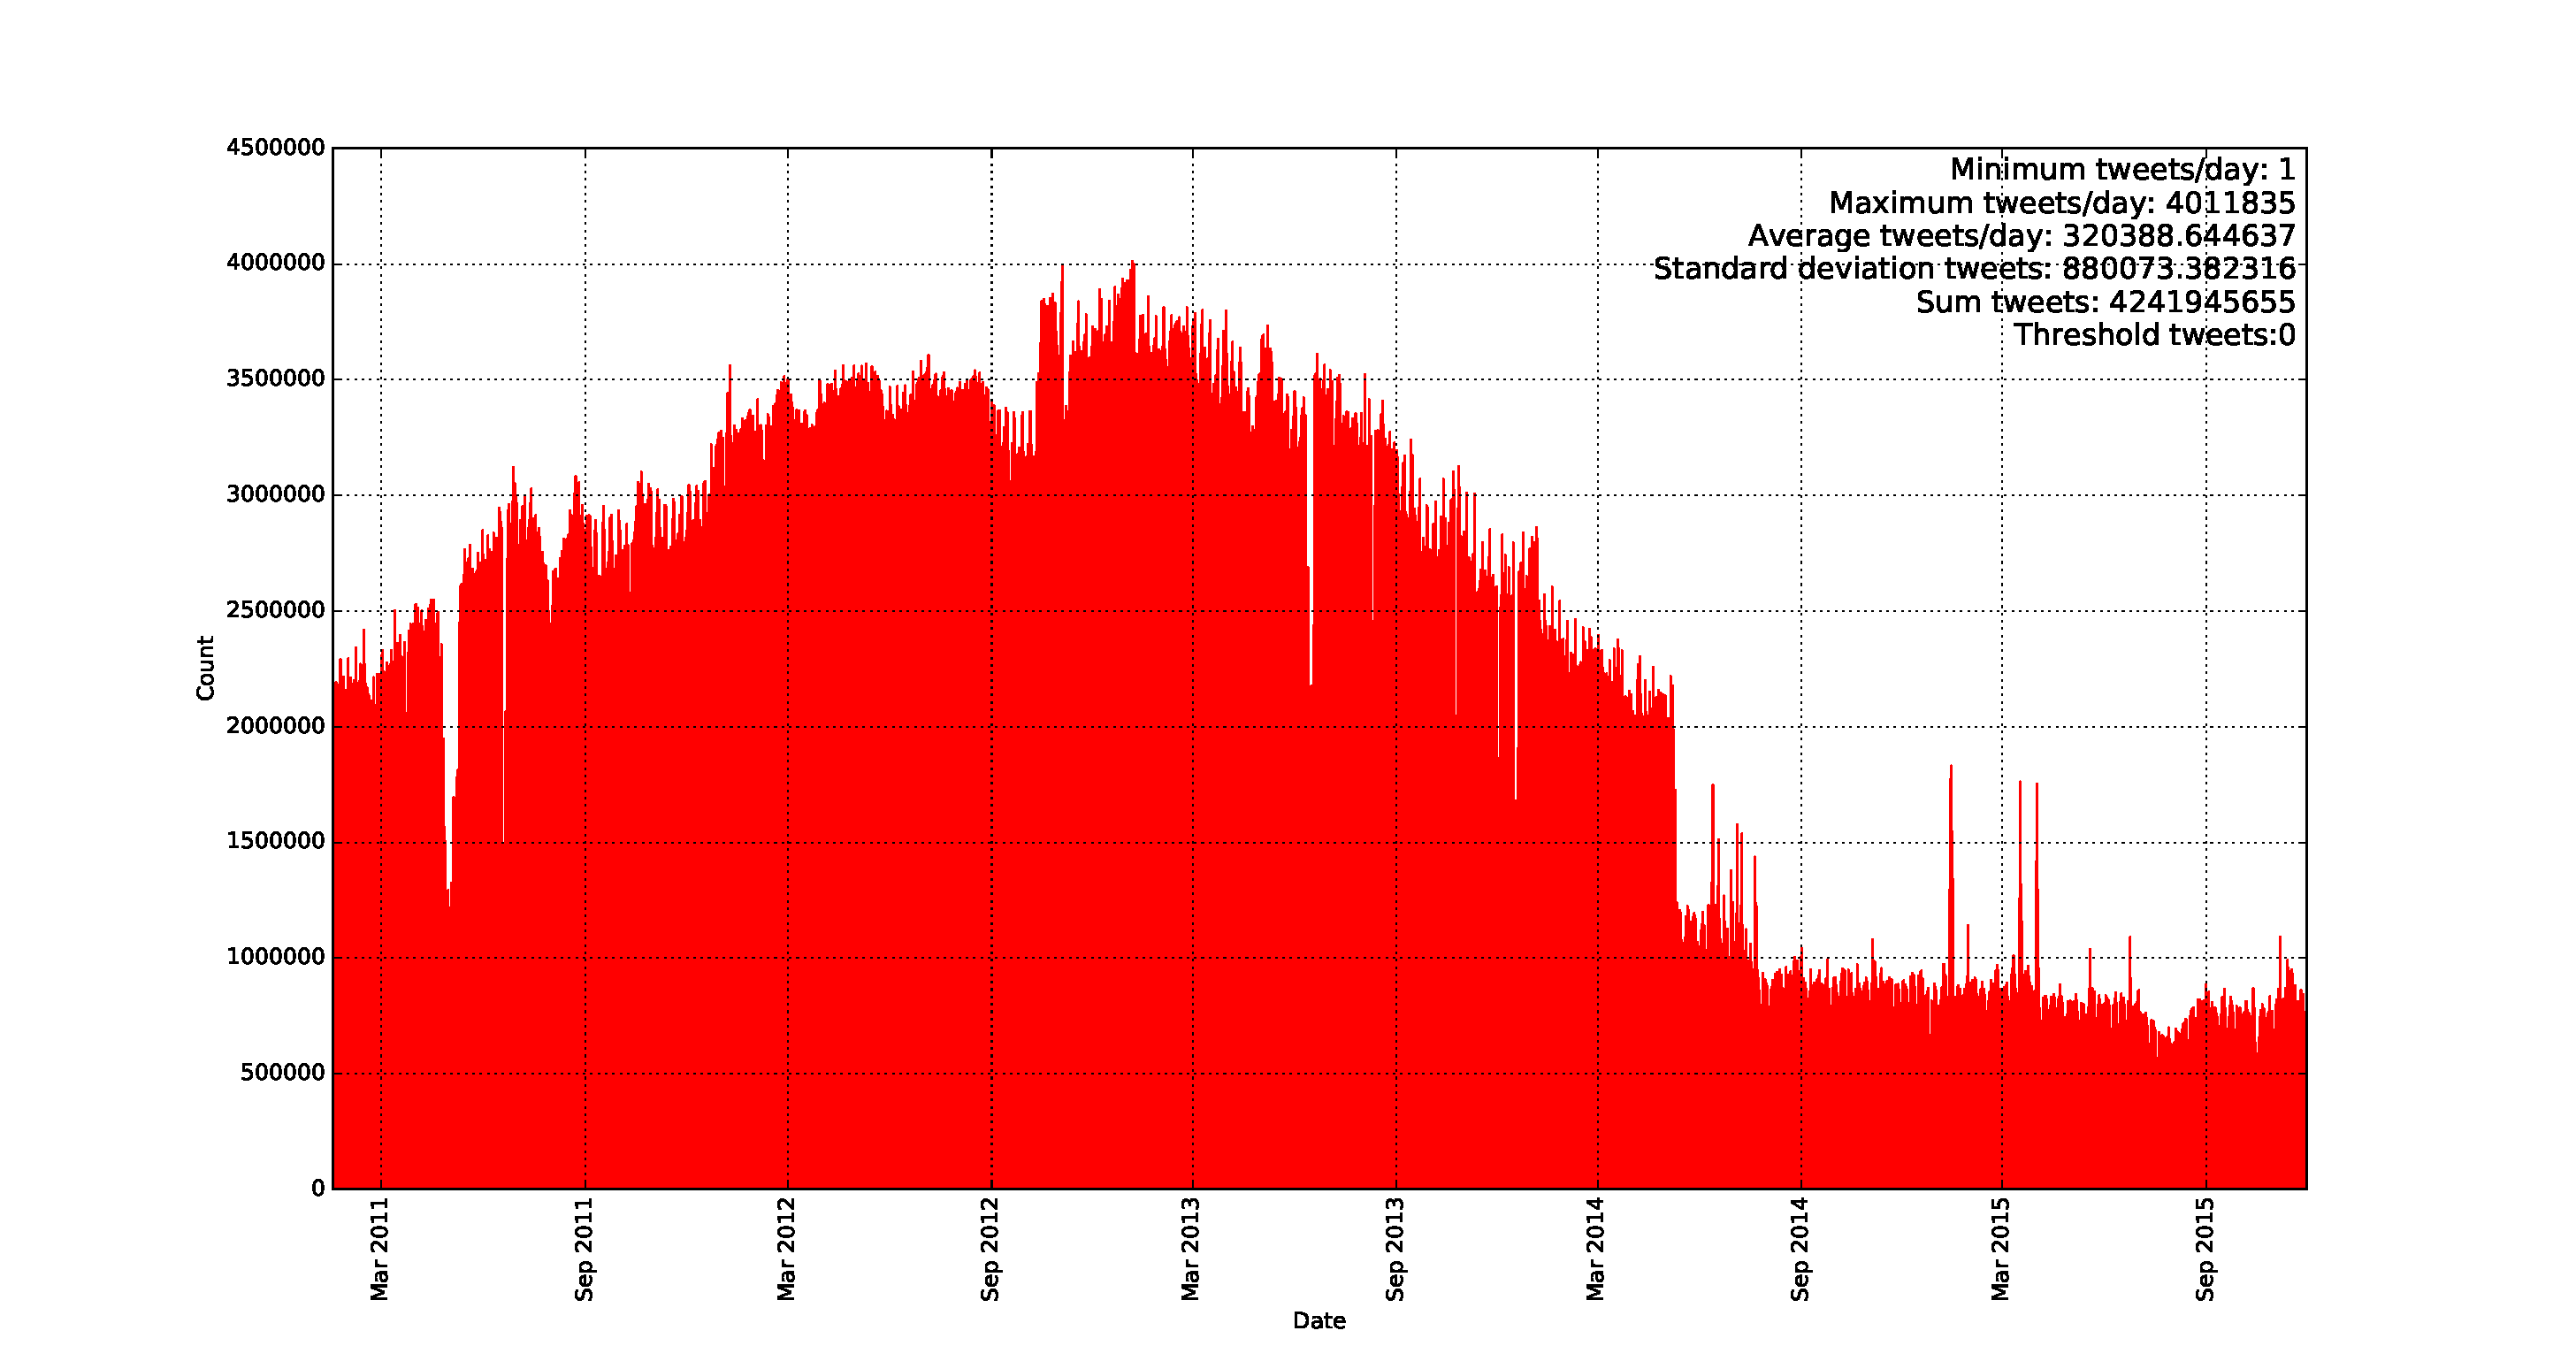
\includegraphics[width=1.2\textwidth]{img/twitter_plot_no_threshold}}
	\caption{The full Twitter dataset: the number of tweets per day.}\label{fig:3}
\end{figure}
\begin{figure}
	\centerline{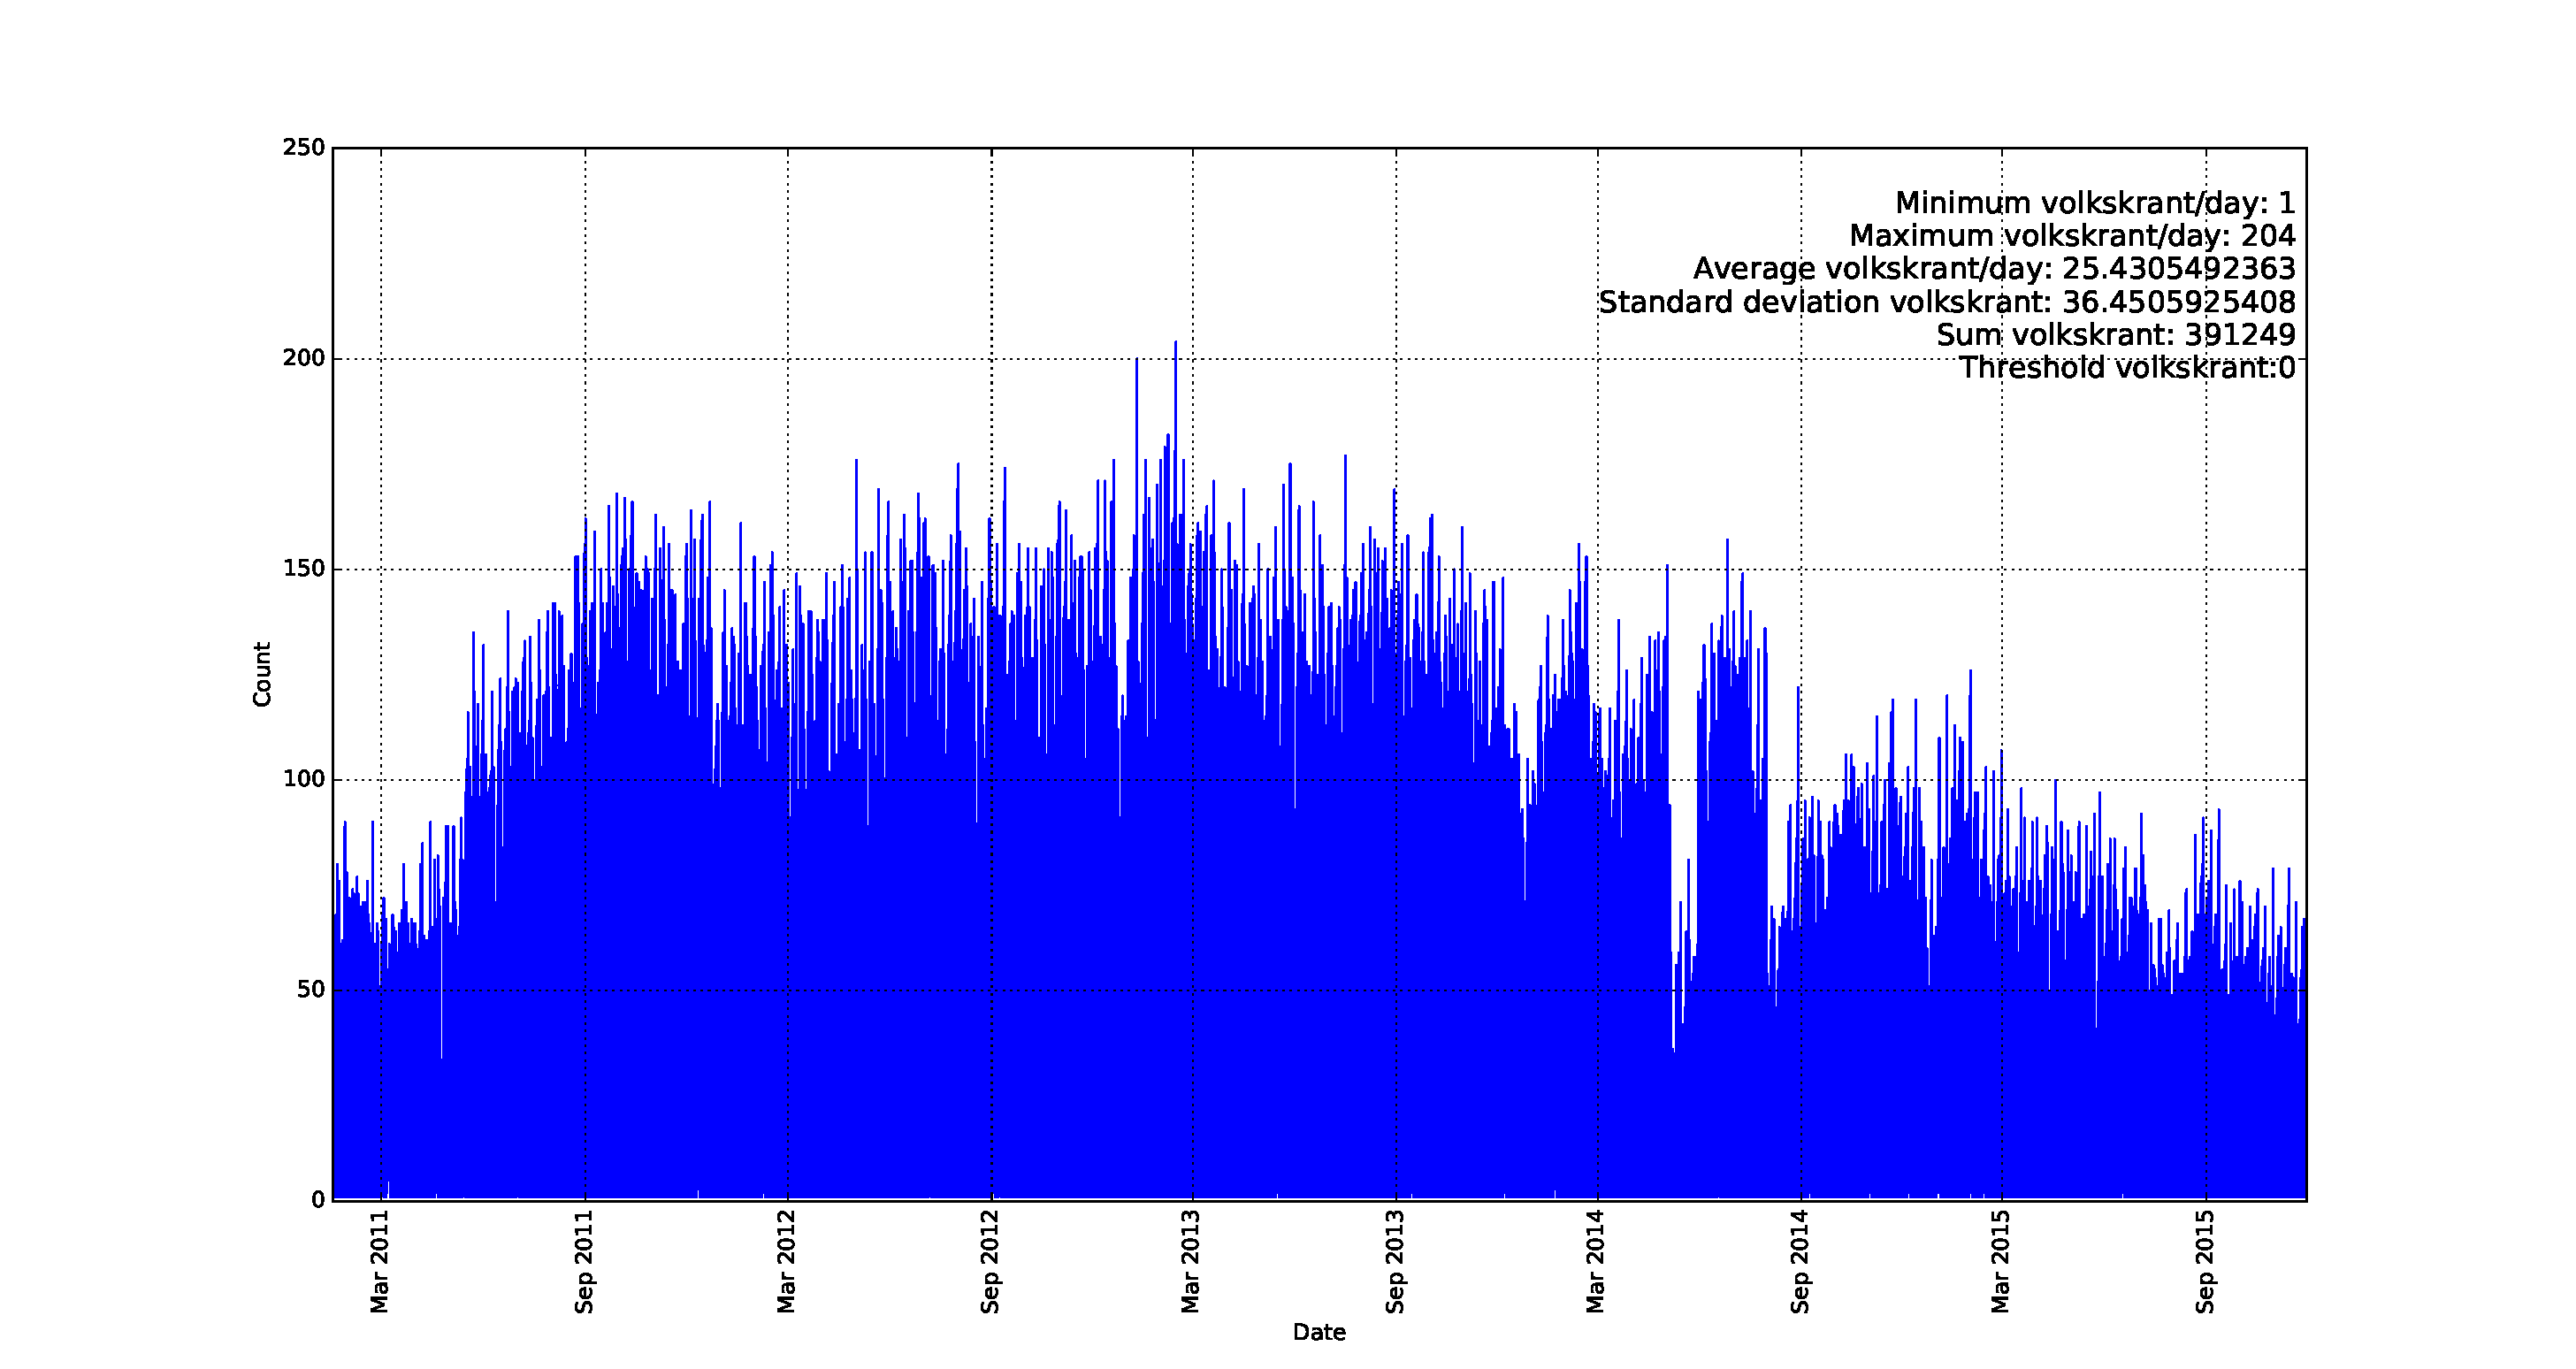
\includegraphics[width=1.2\textwidth]{img/volkskrant_plot_no_threshold}}
	\caption{The full Volkskrant dataset: the number of articles per day.}\label{fig:4}
\end{figure}
\begin{figure}
	\centerline{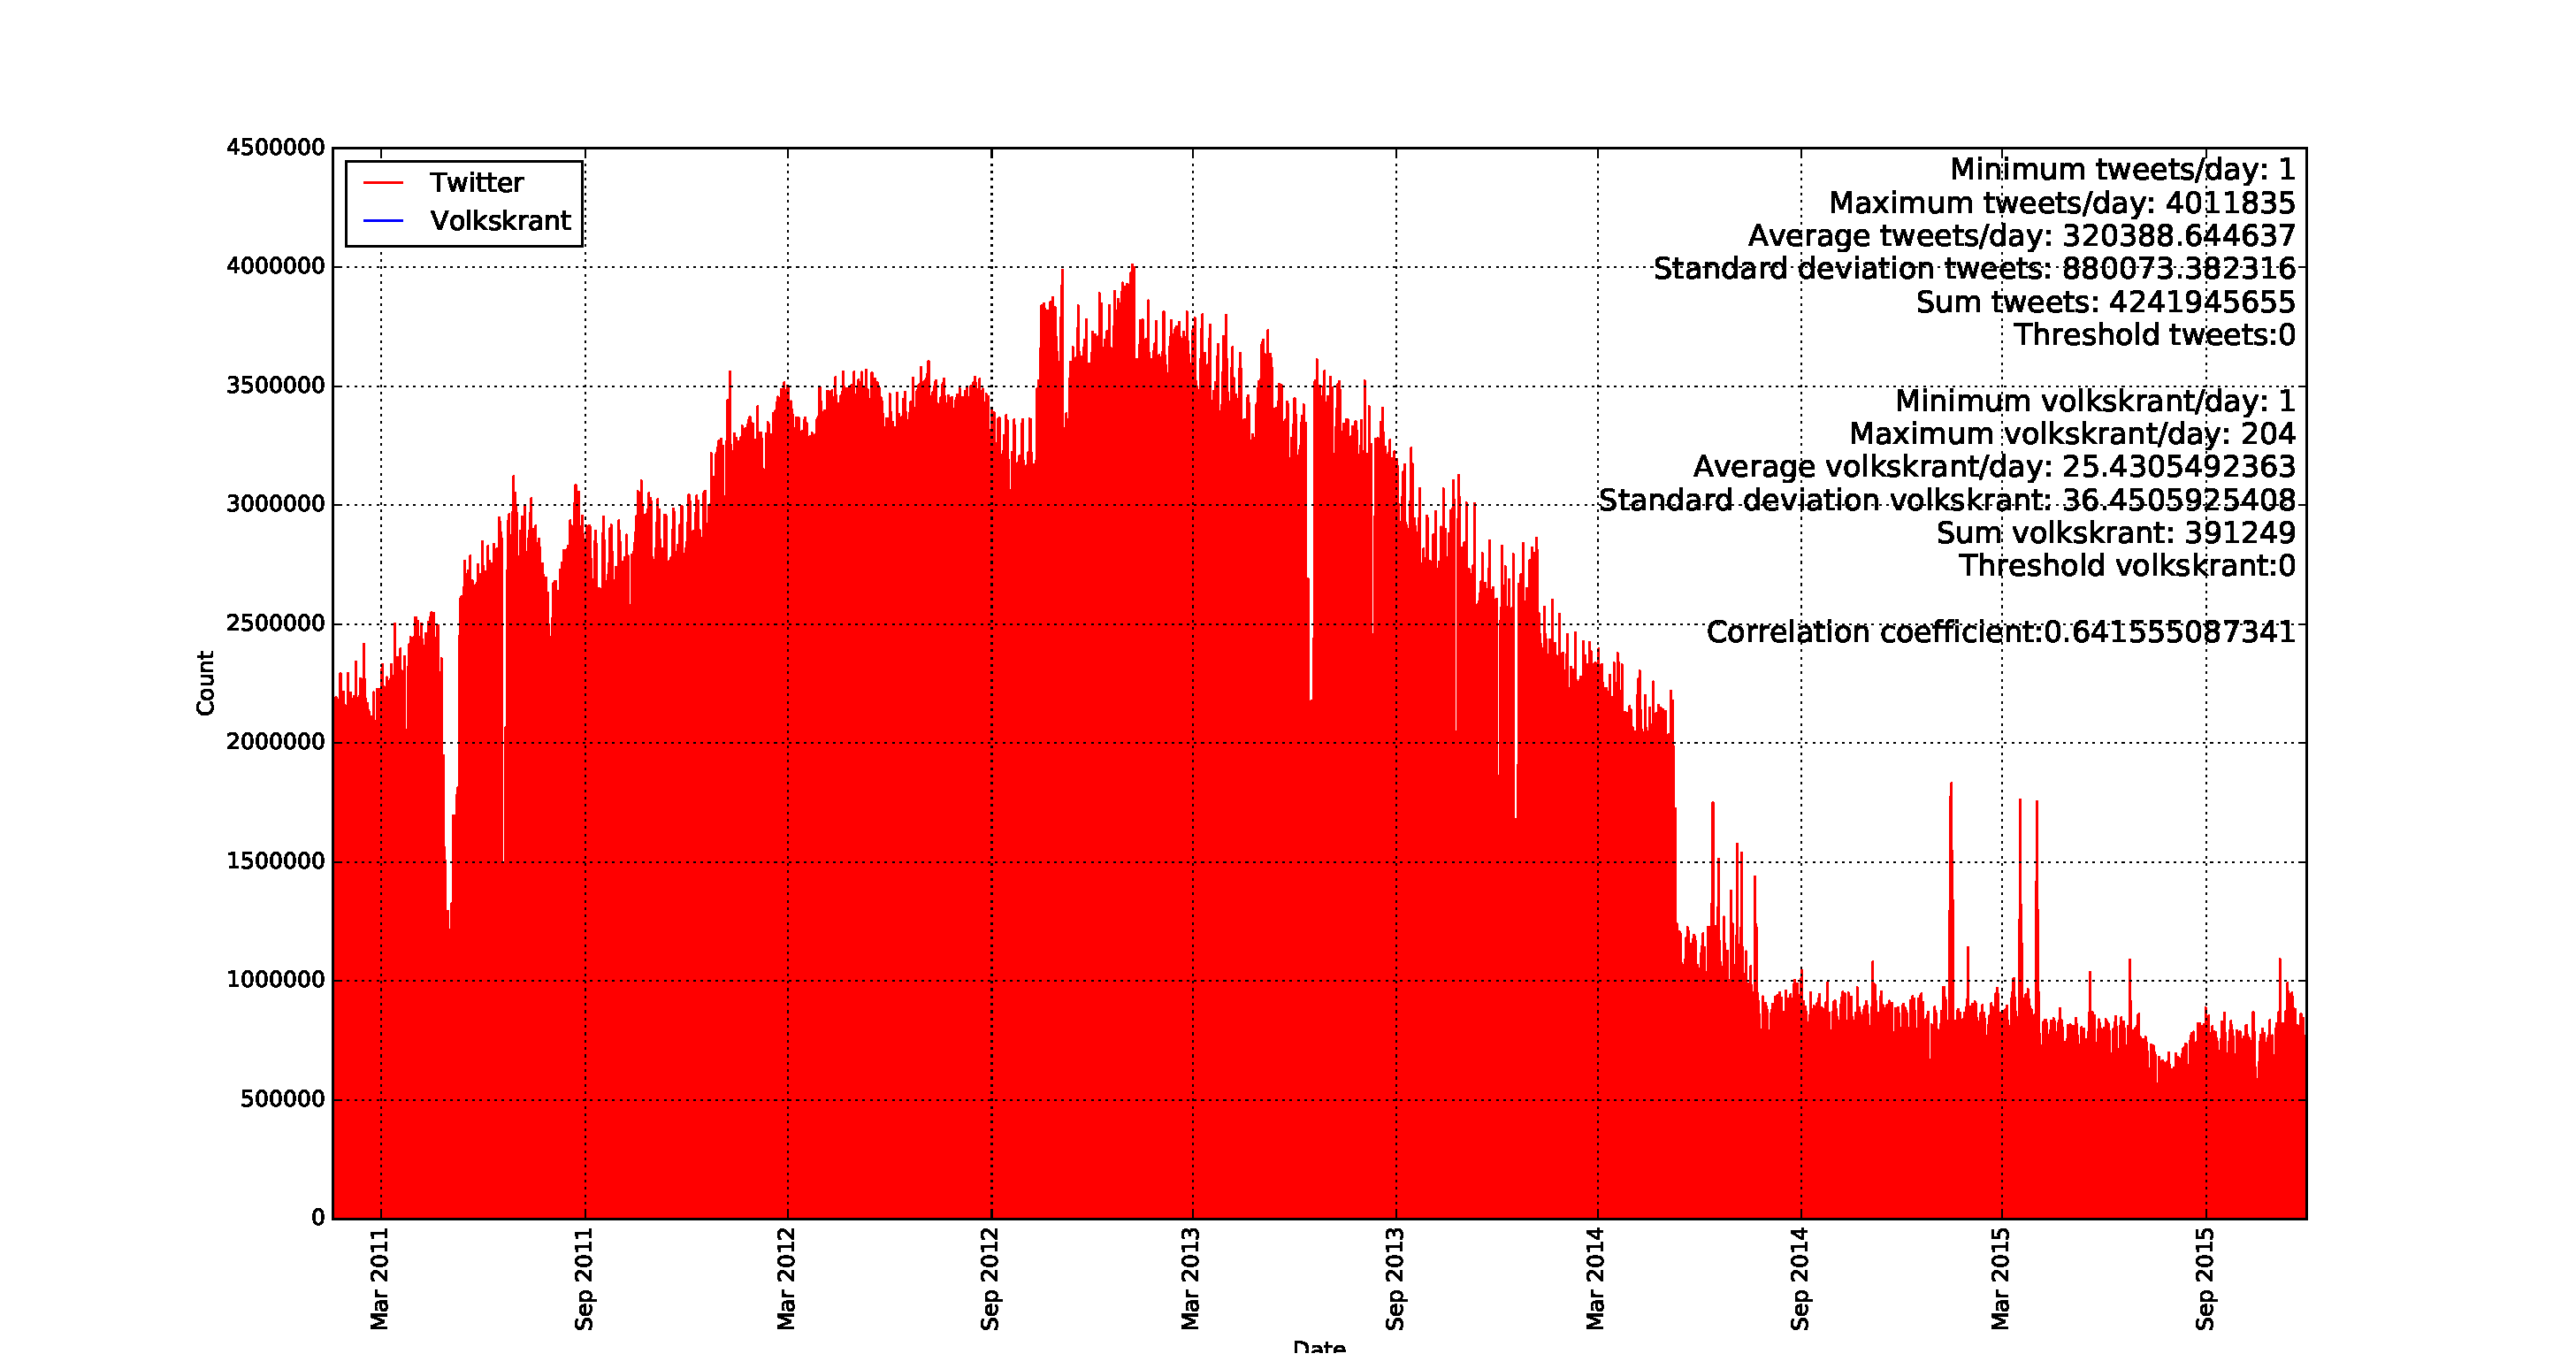
\includegraphics[width=1.2\textwidth]{img/volkskrant_twitter_plot_no_threshold}}
	\caption{The Twitter and Volkskrant datasets, with statistics.}\label{fig:7}
\end{figure}

\begin{figure}
	\includegraphics[width=\textwidth]{img/twitter_plot_threshold}
	\caption{The number of climate related tweets per day.}\label{fig:5}
\end{figure}
\begin{figure}
	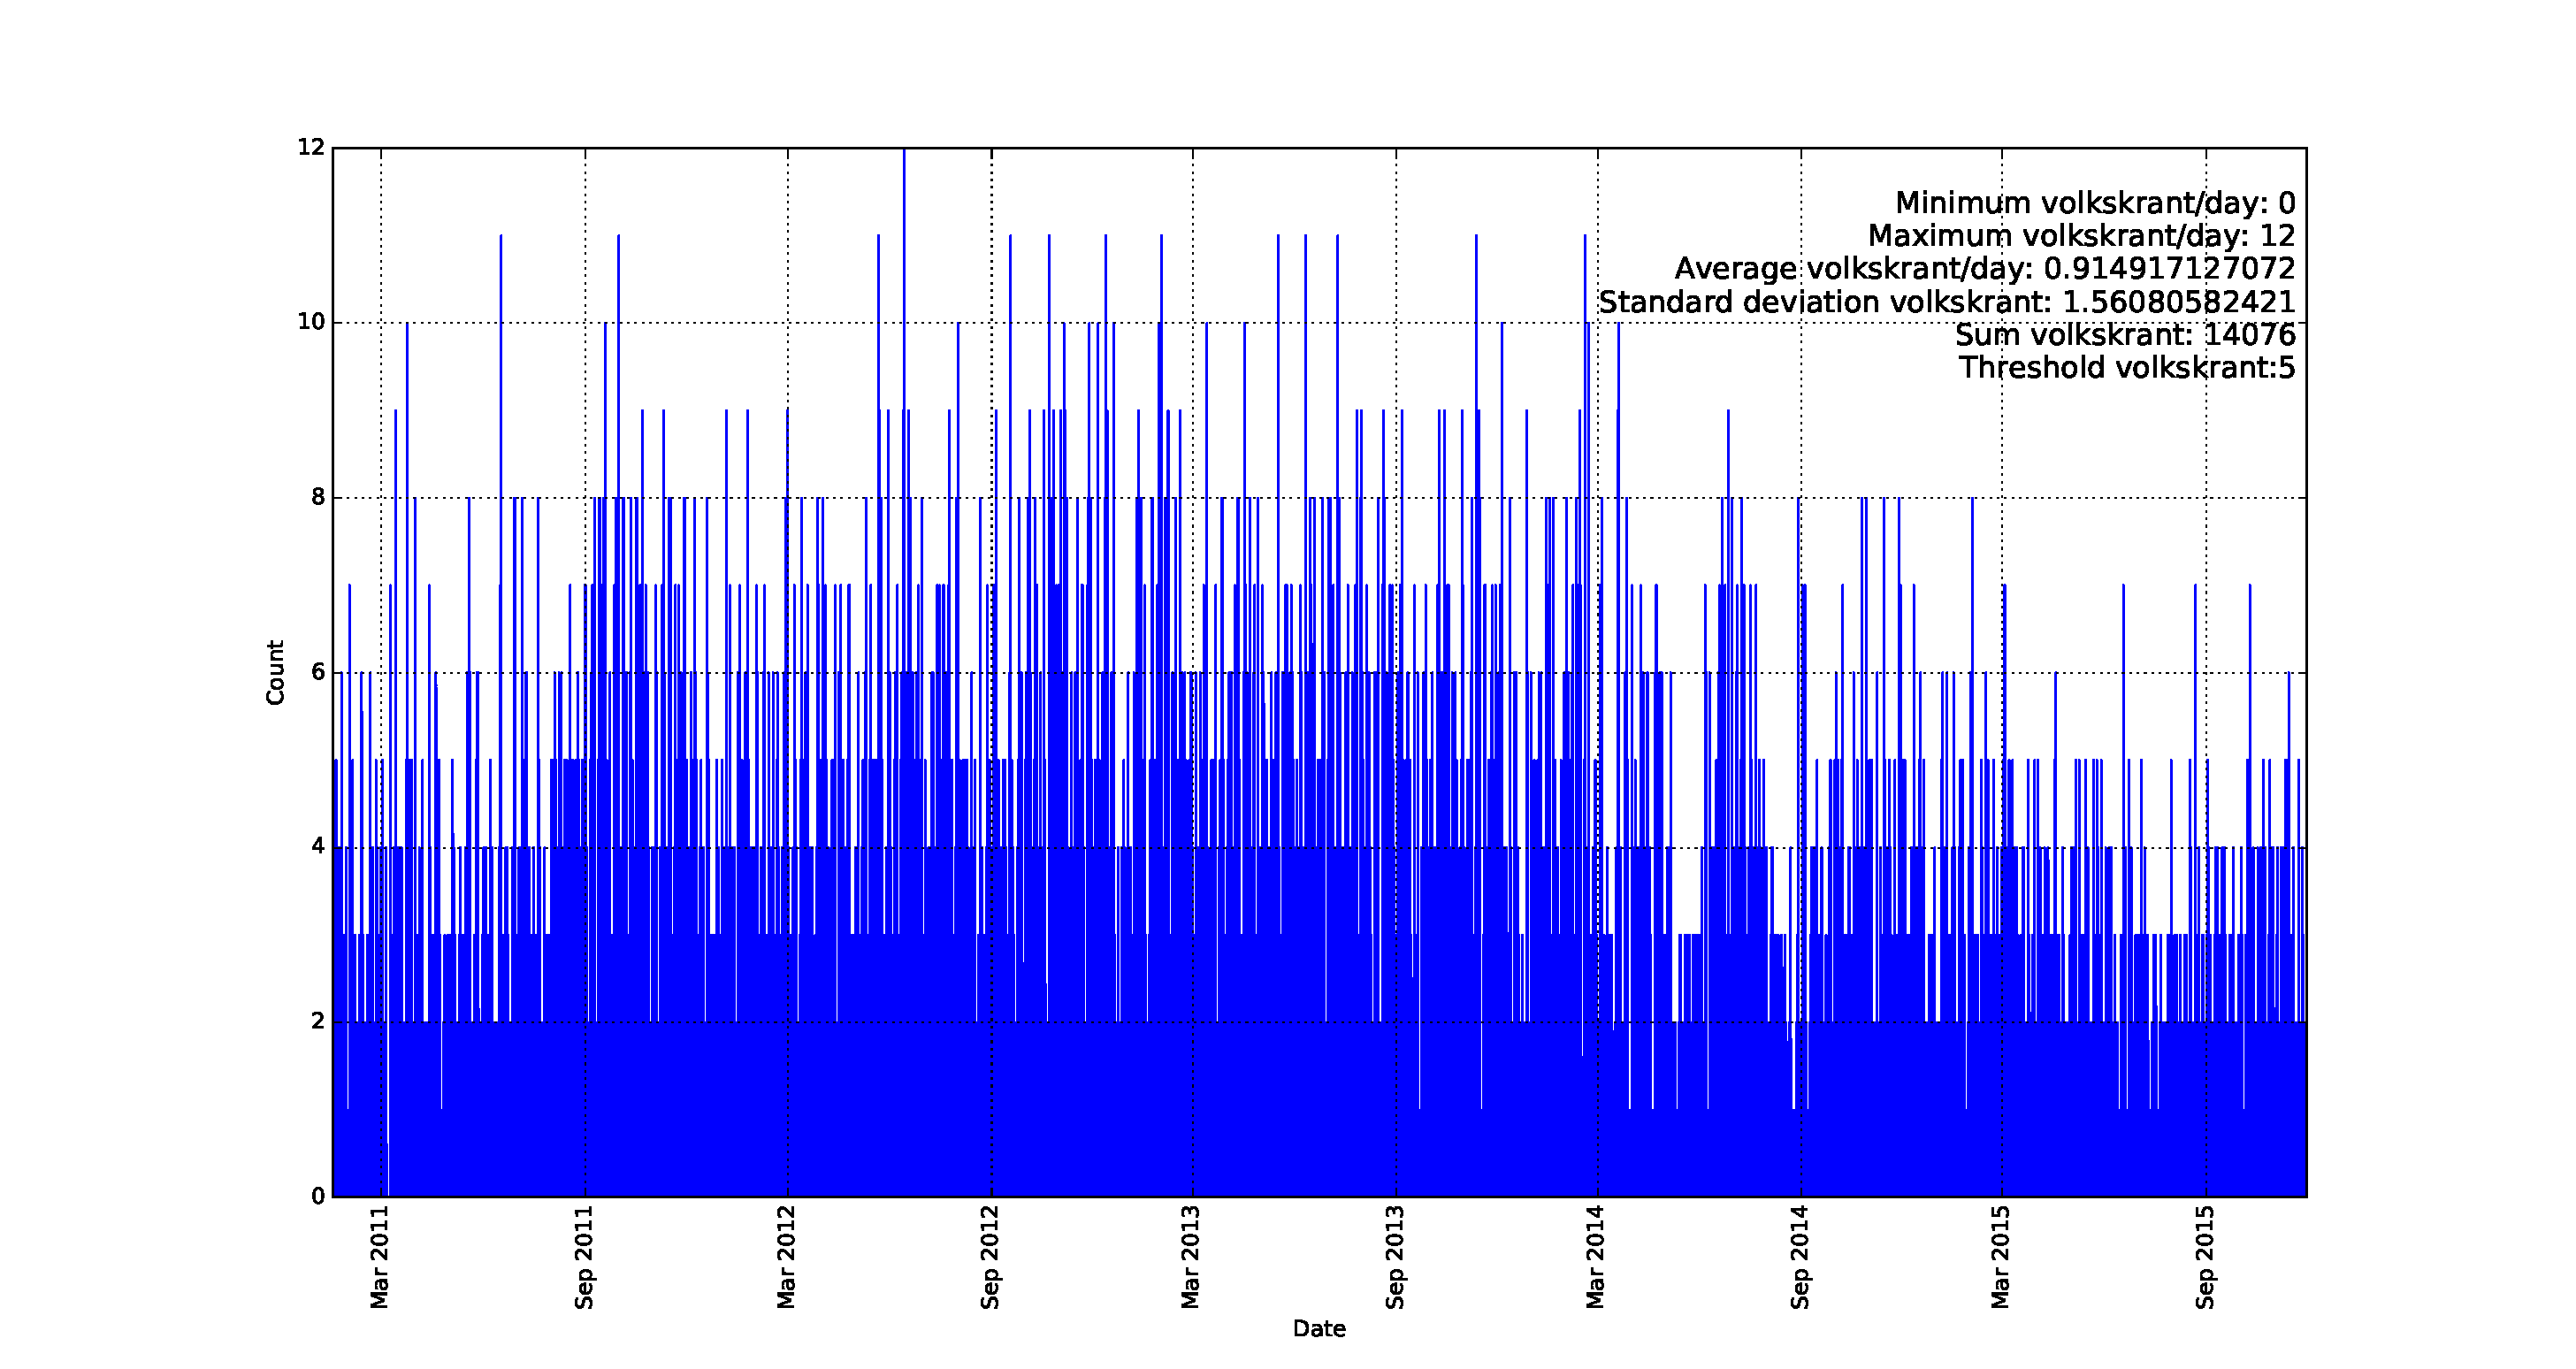
\includegraphics[width=\textwidth]{img/volkskrant_plot_threshold}
	\caption{The number of climate related Volkskrant articles per day.}\label{fig:6}
\end{figure}
\begin{figure}
	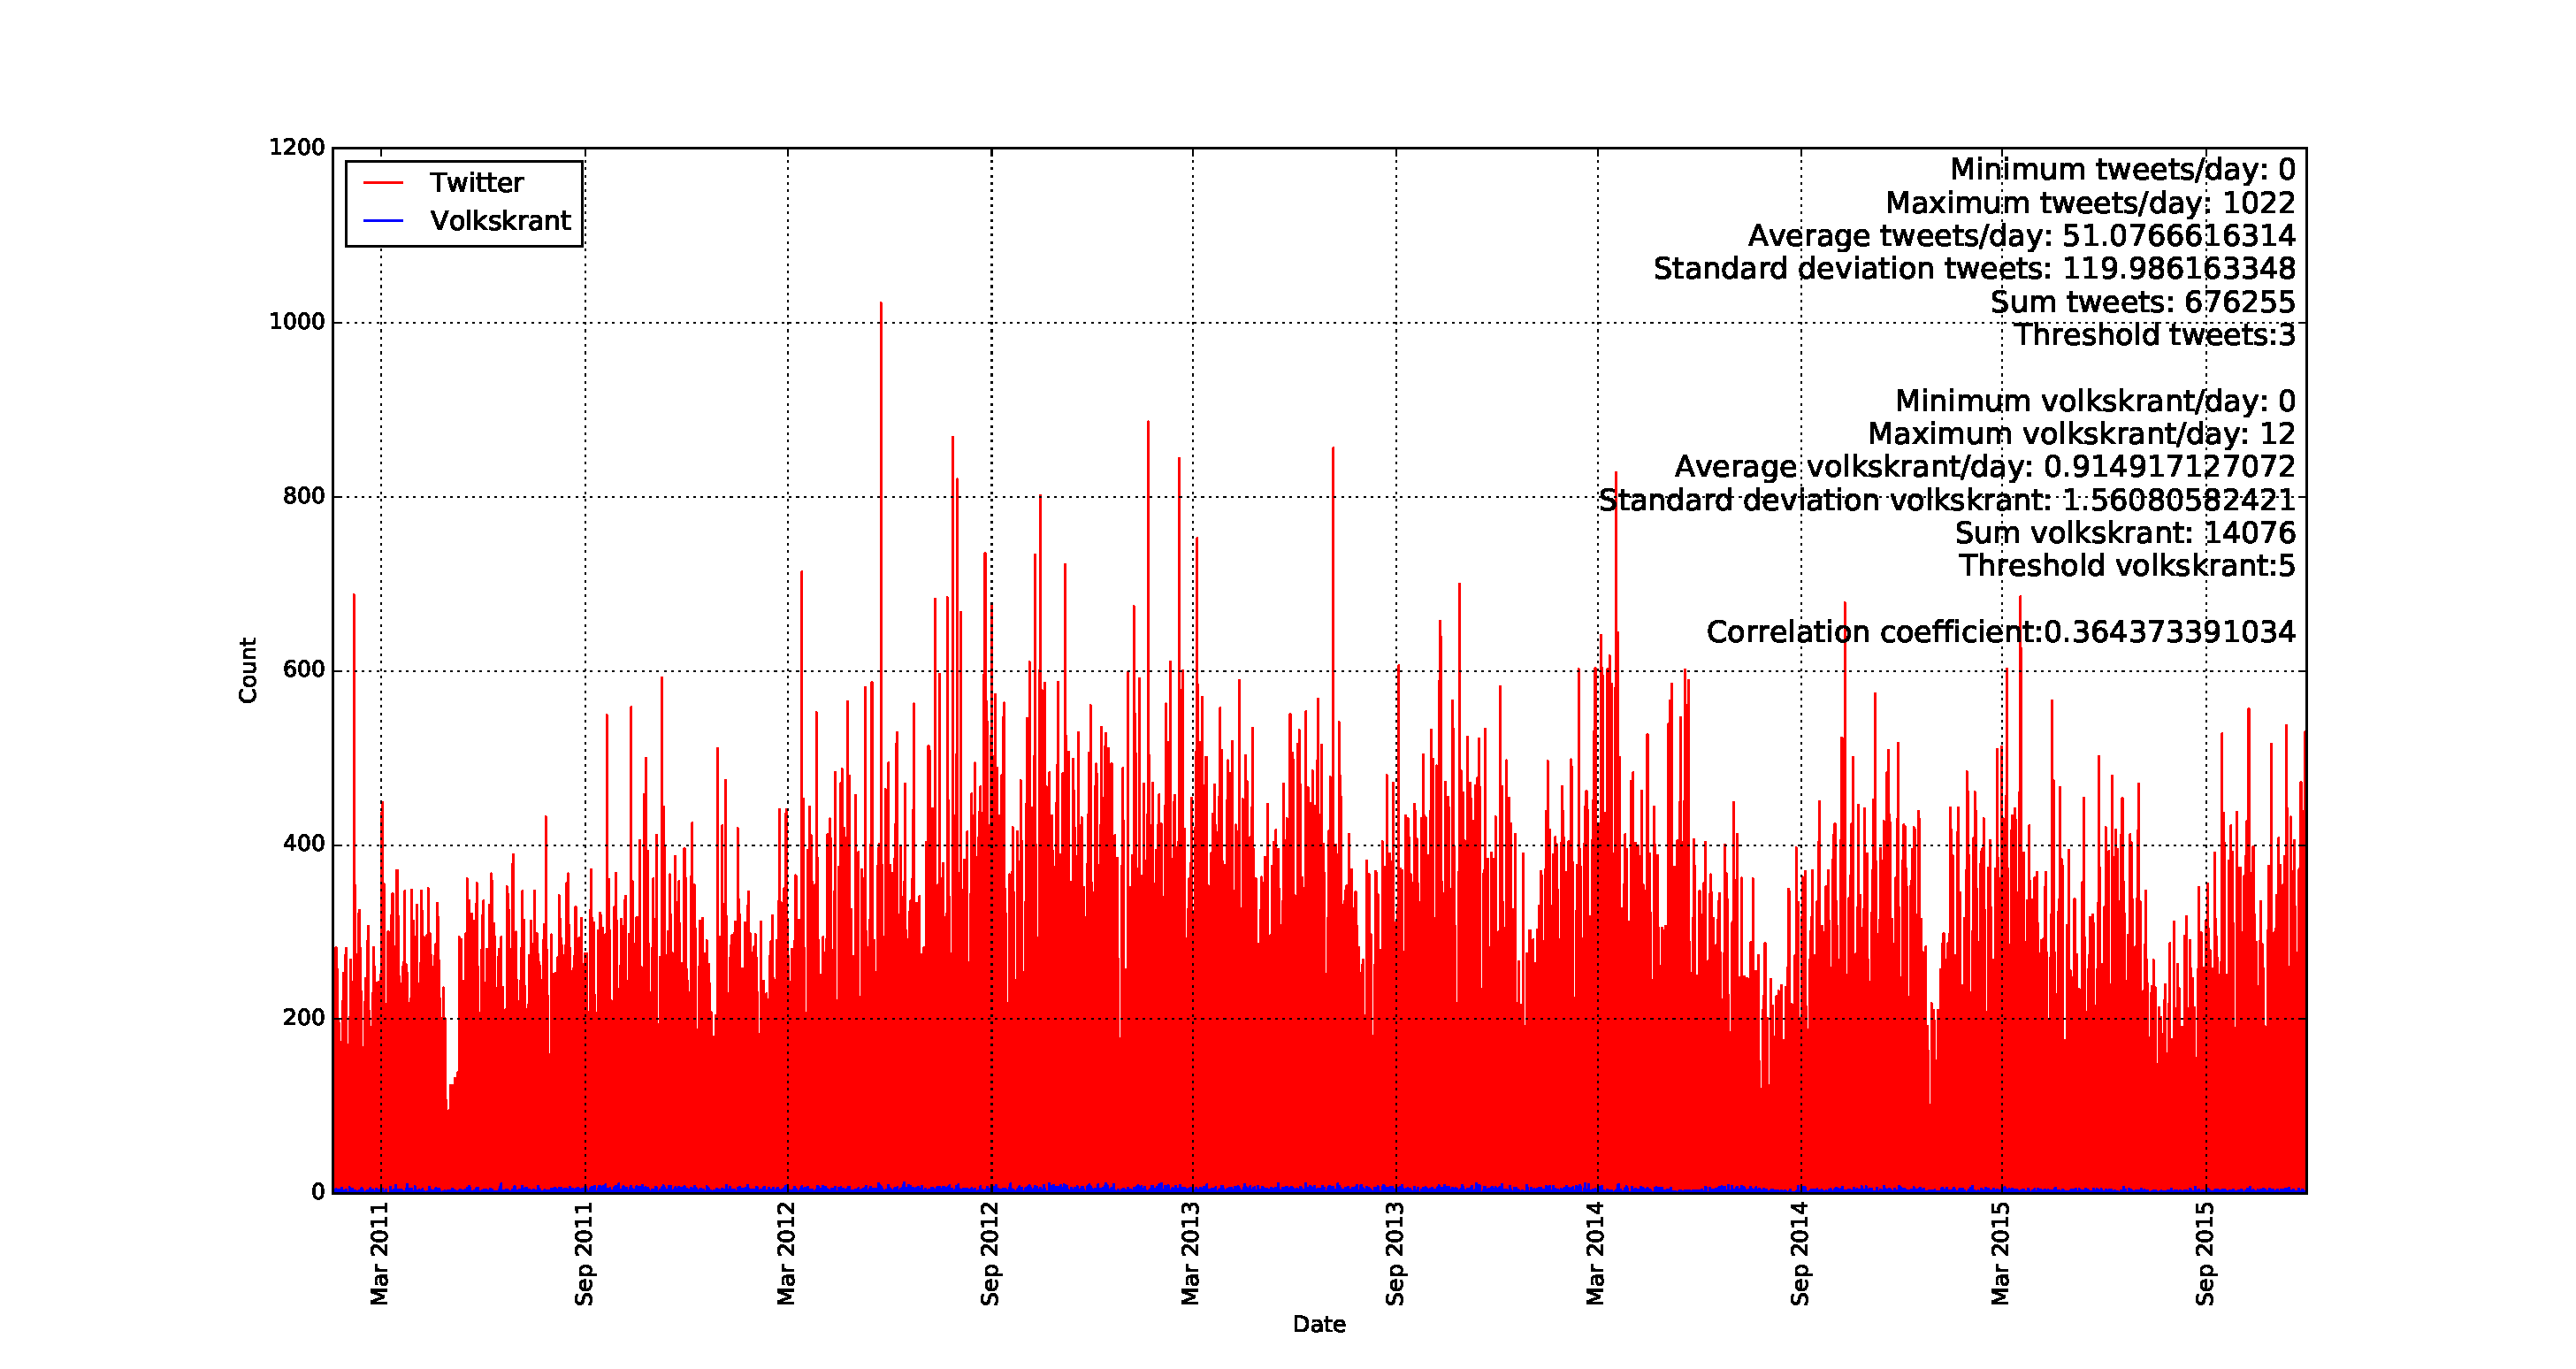
\includegraphics[width=\textwidth]{img/volkskrant_twitter_plot_threshold}
	\caption{The number of climate related tweets and Volkskrant articles per day, with statistics.}\label{fig:8}
\end{figure}

\newpage

\section{References}

\begin{itemize}
	\item[$\bullet$] [1] IPCC, 2007: Climate Change 2007: Synthesis Report. Contribution of Working Groups I, II and III to the Fourth Assessment Report of the Intergovernmental Panel on Climate Change [Core Writing Team, Pachauri, R.K and Reisinger, A. (eds.)]. IPCC, Geneva, Switzerland, 104 pp
	
	\item[$\bullet$] [2] Tan, C. K., Ogawa, A., \& Matsumura, T. (2008). Innovative climate change communication: team minus 6\%. Global Environment Information Centre (GEIC), United Nations University (UNU), 53-70.
	
	\item[$\bullet$] [3] Sampei, Y., \& Aoyagi-Usui, M. (2009). Mass-media coverage, its influence on public awareness of climate-change issues, and implications for Japan’s national campaign to reduce greenhouse gas emissions. Global Environmental Change, 19(2), 203-212.
	
	\item[$\bullet$] [4] Raymond A. Harder, Steve Paulussen \& Peter Van Aelst (2016) Making
	Sense of Twitter Buzz. Digital Journalism, 4:7, 933-943, DOI: 10.1080/21670811.2016.1160790
	
	\item[$\bullet$] [5] Becker, B., Larson, H., Bonhoeffer, J., Van Mulligen, E., Kors, J., Sturkenboom, M., (2016), Evaluation of a multinational, multilingual vaccine debate on Twitter. Volume 34, Issue 50, 7 December 2016, Pages 6166-6171, DOI: 10.1016/j.vaccine.2016.11.007
	
	\item[$\bullet$] [6] An, X., Ganguly, A., Fang, Y., (2014), Tracking Climate Change Opinions from Twitter Data
	
	\item[$\bullet$] [7] Tjong Kim Sang, E., Van den Bosch, A., Dealing with big data: The case of Twitter, Computational Linguistics in the Netherlands Journal 3 (2013) 121-134.
	
	
\end{itemize}

\newpage

\section{Appendix}

\subsection{Terms}
The list of terms in both English and Dutch. 

\textsc{\textbf{English}} \\\textit{English Agriculture Alternative Applied Science Awareness Raising Balance Behavior Change Biodiversity Bioenergy Biomass Biomimicry Brundtland Commission Building Carbon Offset Catalyze Change Change Management City Civil Climate Coastal Collaboration Commissioning Community Community Health Complex Systems Conserve Conservation Conservation Biology Corporate Social Responsibility Cost Benefit Analysis Cradle to Cradle Culture Deforestation Design Development Disaster Discrimination Diversity Ecological Ecology Economic Ecosystem Efficiency Energy Engaged Scholarship Engagement Entrepreneurship Environment Externality Equality Equity Farming Finance Food Food Systems Food Chain Footprint Future Gender Geothermal Global Globalization Governance Green Greenhouse Gas Growth Human Condition Human Rights Human-Environment Interactions Innovation Innovative Integrated Interconnections Interdisciplinary Invest Justice Land Landscape LEED (Leadership in Energy and Environmental Design) Life Life Cycle Local Marine Materials Minority Modernization Movements Multidisciplinary Natural Systems Nature Nutrition Outreach Partnership Photovoltaic Planning Policy Political Population Poverty Problem Based Prosperity Public Public Health Race Recycle Recycling Renewable Resilience Resources Revolving Fund Rights Rural Sea Level Social Solar Solutions Stakeholder Stewardship Suburbanization Supply Chain Sustainable Sustainability Systems Dynamics Systems Thinking Technology Three Legged Stool Three Pillars Tradeoffs Transdisciplinary Transformation Transit Transparency Transportation Triple Bottom Line Underserved Unintended Consequences Urban Urbanization Water Welfare Wind Energy Women}\\
	
\textsc{\textbf{Dutch}} \\\textit{Landbouw Alternatief Toegepast Wetenschap Bewustmaking Balans Gedrag Verandering Biodiversiteit Bioenergie Biomassa Biomimicry Brundtland Commissie Koolstof Offset Katalyseren Verandering Stad Civiel Klimaat Kust Samenwerking Gemeenschap Gezondheid  Complexe Systemen Conserveren Biologie Maatschappelijk Kosten Baten Analyse Cultuur Ontbossing Design Ontwikkeling Ramp Discriminatie Diversiteit Ecologie Ecologisch Economisch Economische Ecosysteem Efficiëntie Energie Toegeweid Beurs Ondernemerschap Omgeving Gelijkheid Billijkheid Landbouw Financiën Voedel Voedselsystemen Voedselketen Spoor Toekomst Geslacht Geothermisch Geothermische Globaal Globalisering Bestuur Groen Broeikas Gas Groei Menselijk Voorwaarde Rechten Human Innovatie Innovatief Geïntegreerd Aansluitingen Interdisciplinair Investeren Justitie Land Landschap Leiderschap Leven Levenscyclus Lokale Marine Materialen Minderheid Modernisering Bewegingen Multidisciplinair Multidisciplinaire Natuurlijk Natuurlijke Systemen Natuur Voeding Overtreffen Partnerschap Photovoltaisch Ruimtelijk Beleid Politiek Politieke Bevolking Armoede Probleem Gebaseerd Welvaart Publiek Volksgezondheid Race Recycle Recycling Hernieuwbaare Hernieuwbaar Veerkracht Bronnen Draaibaar Fonds Rechten Landelijk Zeeniveau Sociale Zon Oplossingen Belanghebbende Stewardship Suburbanisatie Toevoer Ketting Duurzaamheid Duurzaam Duurzame Dynamieken Denken Technologie Afwegingen Transdisciplinair Transformatie Doorvoer Transparantie Transport Planet Ondergeserveerd Onbedoeld Onbedoelde Gevolgen Stedelijk Verstedelijking Water Welzijn Wind Energie}
\end{document}